%!TeX ts-program = xelatex
%!TeX encoding = utf-8 Unicode
\documentclass[ieeetran]{article}
\usepackage{amsmath, amssymb}
\usepackage{graphicx}



\title{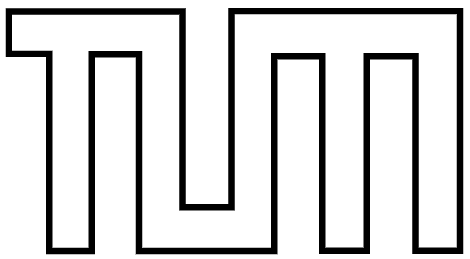
\includegraphics[width=0.43\textwidth]{tumlogo}\hspace{2ex}
\includegraphics[width=0.25\textwidth]{maxlogo}\vspace{1ex}\\ \large \textbf{Max Planck Computing and Data Facility \\Chair of Computer Architecture and Parallel Systems} \vspace{10ex}\\ \huge Tensorflow \vspace{2ex}\\
\large Seminar: Efficient Programming of HPC Systems \\Frameworks and Algorithms\vspace{15ex}}


\author{Efe Kamasoglu}


\begin{document}

\maketitle

\pagebreak

\tableofcontents

\pagebreak

\addcontentsline{toc}{section}{Abstract}
\section*{Abstract}



\pagebreak


\section{Introduction} % (fold)
\label{sec:introduction}
TensorFlow is a free and open-source framework developed by Google Brain, which finds its application widely in the field of machine learning and artificial intelligence. It is used to build and train large-scale models according to the client's preferences and provided data sets. In order to train a model, TensorFlow carries out several computations by mapping them onto a variety of hardware, such as mobile devices or HPC clusters consisting of multiple computational units with hundreds of GPUs. Those computations are represented in a "directed dataflow graph"\footnote{Martin Abadi, Ashish Agarwal, ..., "TensorFlow: Large-Scale Machine Learning on Heterogeneous Distributed Systems," November 9, 2015, p.\ 1, para.\ 2} as a whole, which is then compiled statically or dynamically depending on the version of Tensorflow. 
\\ \\To construct such graph, a client needs to create a session which is an interface with methods of its own. Through those methods, the client can introduce his data set to Tensorflow's system, define his model and its specifications. A graph is typically composed of the following:
\begin{itemize}
  \item \textit{Node:} A node has zero or more inputs and zero or more outputs. It is an instantiation of an operation.
\item \textit{Edge:} Data flows through the edges from one node to another. There are also edges which are not for the dataflow, but for control dependencies between different nodes; e.g., execution order of the concerning operations.
\item \textit{Operation:} An operation represents a computation such as addition or matrix dot product.
\item \textit{Tensor:} Tensors are multidimensional arrays describing the data. They flow into the nodes as inputs through the edges of a graph.
\item \textit{Kernel:} A kernel is an implementation of an operation.
\item \textit{Device:} Devices are computational units on a machine that are utilized by TensorFlow's system to execute kernels. (e.g.\ GPUs)
\end{itemize}
Client can either execute all or a part of the graph with the help of the session, where he interacts with the processes that regulate access to devices. In addition to that, TensorFlow system itself has different implementations for execution mechanisms both for single- and multiple-device systems.  
\section{Execution of a Graph} % (fold)
\label{sec:execution_of_a_graph}
Each implementation follows the same standard (Fig.\ 1): Client process calls the master process through the session interface to ignite the execution. An arbitrary number of worker processes, each of which executes a subgraph, are called by the master process. Each worker is responsible for one or more devices. Master distributes the operations as well as the data tensors to the workers. Also, a worker can fetch the data by itself directly from storage system to the device's memory. The number of workers depends on the architecture of the system. As we are going to focus on efficiency, scalability and portability of TensorFlow in terms of HPC systems, we have to take a closer look at the distributed implementation.
\begin{figure}[h!]
  \centering
 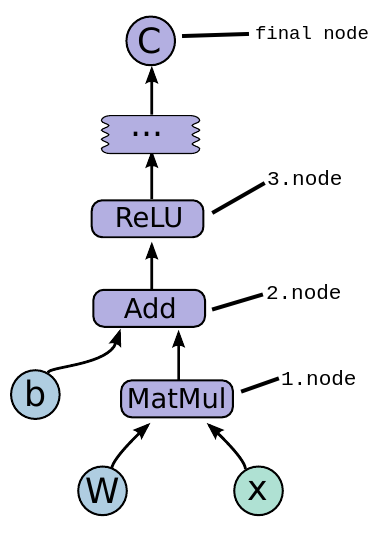
\includegraphics[width=0.2\linewidth]{graph}
\caption[placeholder]{Subgraph example for a neural network\footnotemark}  

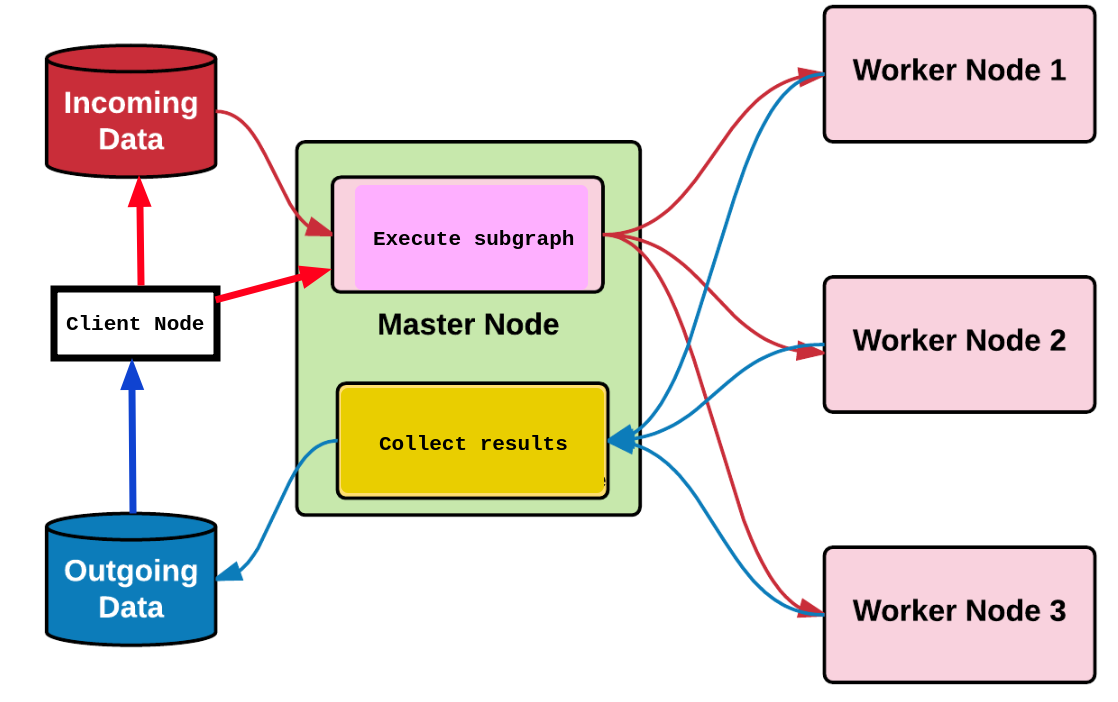
\includegraphics[width=0.5\linewidth]{executionofgraph}
 \caption[placeholder]{Master and Worker processes of a distributed system\footnotemark} 
  \label{fig:executionofgraph}
\end{figure}
\addtocounter{footnote}{-2}
\stepcounter{footnote}\footnotetext{Martin Abadi, Ashish Agarwal, ..., "TensorFlow: Large-Scale Machine Learning on Heterogeneous Distributed Systems," November 9, 2015, p.\ 3, fig.\ 2}
\stepcounter{footnote}\footnotetext{https://www.oreilly.com/api/v2/epubs/9781787281349/files/assets/Ch09-Fig11.png}
\subsection{Distributed (Multiple-Device) Implementation} % (fold)
\label{subsec:multiple_device_execution_of_a_graph}
If we consider a system with a single device, the execution is fairly simple: A worker process is created for the device. Data is placed into the memory and all the nodes are mapped to the same device. The device executes them in an order according to the control dependencies between the nodes.
\\ \\However, in the case of multiple devices, we encounter a handful of programming challenges as to resource management, mapping of the nodes to the devices and intercommunication between the devices in terms of data transfer.







\end{document}
